\documentclass[aspectratio=169,compress]{beamer}
\usetheme[university=bs,faculty=standard]{fibeamer}
\usepackage[utf8]{inputenc}
\usepackage[
  main=english
]{babel}        %% typeset as follows:
%%
%%   \begin{otherlanguage}{italian}   ... \end{otherlanguage}
%%
%% These macros specify information about the presentation
\title{All Set: Bringing Static Types to Elixir}
\subtitle{\mbox{ }\vspace{6mm}
} %% title page.
\author{Giuseppe CASTAGNA {\small(CNRS, Université Paris Cité)}
\hfill\parbox[t]{.2\textwidth}{
\footnotesize\it
Elisir di sì perfetta,\\[-1.5mm]
di sì rara qualità,\\[-1.5mm]
ne sapessi la ricetta,\\[-1.5mm]
conoscessi chi ti fa!\\[-0.5mm]
{\upshape\tiny --- G.~Donizetti, \textit{L'elisir d'amore}}
}\\[-8mm]
Guillaume DUBOC {\small(University of Bristol)}}
%% These additional packages are used within the document:
\usepackage[overlay,absolute,
%showboxes
]{textpos}
\usepackage{ragged2e}  % `\justifying` text
\usepackage{booktabs}  % Tables
\usepackage{tabularx}
\usepackage{tikz}      % Diagrams
\usetikzlibrary{calc, shapes, backgrounds}
\usepackage{amsmath, amssymb}
\usepackage{url}       % `\url`s
\usepackage{listings}  % Code listings
\usepackage{setup}
\usepackage{ulem}
\usepackage[cal=boondox,  % heavily sloped
            scr=esstix]   % slightly sloped
           {mathalpha}
\newtagform{purple}{\color{purple}(}{)}
%\frenchspacing

\newcommand{\struct}[1]{\textcolor{lightblue}{#1}}
% Beamer customization%%
\setbeamerfont{frametitle}{shape=\bf,size=\LARGE}
\addtobeamertemplate{frametitle}{\vspace*{-.4cm}}{\vspace*{0.2cm}}

\newenvironment<>{myblock}[1]{%
  \setbeamercolor{block title}{fg=cadmiumgreen,bg=white}%
  \setbeamercolor{block body}{fg=black,bg=white}%
  \setbeamerfont{block title}{size=\large,shape=\bf}
  \begin{block}#2{{#1}\vspace{-1.5mm}}}{\end{block}}

\setbeamerfont{section in toc}{size=\small}
\setbeamerfont{subsection in toc}{size=\footnotesize}

%%%% UNCOMMENT THE FOLLOWING LINE TO REMOVE SLIDE NUMBERS
%\setbeamertemplate{footline}{}

\begin{document}
  \frame[c]{\maketitle
    \begin{textblock}{3.6}(11.9,0.75)
      
\includegraphics[width=\textwidth]{images/logo-bristol.pdf}
    \end{textblock}
    \begin{textblock}{14}(1.1,14.9)
      \footnotesize\textcolor{white}{$\lambda$ Func Prog Conf, 14 Oct 2026, Stockholm}
    \end{textblock}}

\section{Set-theoretic types and dynamic languages}
\begin{frame}
\frametitle{Outline} 
\tableofcontents
\end{frame}

%% ----------------------------------------------------------
%%  SLIDE 2 — Why static typing for dynamic languages?
%% ----------------------------------------------------------
\begin{frame}
\frametitle{Why static typing for dynamic languages?}

\vspace{-3mm}
\small
\begin{block}{Static types for dynamic languages}\setlength{\leftmargini}{1.2em}
  \begin{itemize}\setlength{\itemsep}{3pt}
    \item \textbf{Catch bugs early} and enable \textbf{tooling}: completion,
          navigation, safe refactoring
    \item \textbf{Checked documentation}: types state what functions expect and
          return; crucial when code is written by AI and read by programmers
    \item \textbf{Existing solutions fall short}: TypeScript, Flow, Hack are
          language-specific and unsound; rewriting in a typed language takes years
    \item \textbf{Needed}: a type system that is \textbf{sound},
          \textbf{gradual}, \textbf{automated}, and \textbf{open}
  \end{itemize}
\end{block}
\setbeamercolor{block body alerted}{bg=red!8}
\begin{alertblock}{Regulatory compliance}\setlength{\baselineskip}{0.85\baselineskip}
  EU and US regulations increasingly \textbf{require evidence of
  software assurance} (CRA, NIST guidelines, \ldots). A
  \emph{sound} type system is a mechanically verifiable step in that direction,
  also for AI-generated code.
\end{alertblock}

\textbf{\color{darkslateblue}The challenge: dynamic code relies on idioms that classic
type systems cannot describe}

\end{frame}

\subsection{Branching, overloading, and pattern matching}

% language tag in the top right corner of TypeScript code boxes (put at the end of the first line)
\newcommand{\tsLabel}{\hfill\textcolor{gray}{\sffamily{\scriptsize T}{\tiny YPE}{\scriptsize S}{\tiny CRIPT}}}% faked small caps: the sans font (Carlito) has none
\begin{frame}[fragile]\transdissolve
\frametitle{1. Branching and discriminated unions}\vspace{-4mm}
\begin{minted}[fontsize=\normalsize]{typescript}
type Status = "success" | "error";!\tsLabel!
function report(s: Status): number | string {
  if (s === "success") return 200;
  return "failed";
}
\end{minted}
{\small\color{gray}The result is \texttt{number} or \texttt{string} depending on the branch\par}
\pause
\vspace{-2mm}
\begin{minted}[fontsize=\normalsize]{typescript}
type Payment = !\tsLabel!
  | { kind: "card";   cardNo: string }
  | { kind: "paypal"; email: string };
\end{minted}
\vspace{-1mm}%
{\small\color{gray}A \emph{discriminated union}: the field \texttt{kind} tells which variant a payment is\par}
\pause
\begin{exampleblock}{$\Rightarrow$ Union and singleton types are needed}
\pb{"success"}, \pb{"error"}, \pb{"card"}: types with one value;\quad \pb{Status}, \pb{Payment}: their unions
\end{exampleblock}
\end{frame}



\begin{frame}[fragile]\transdissolve
\frametitle{2. Overloading}
\structure{\bf Aka \emph{ad hoc} polymorphism: functions that execute different code on arguments of different types}

\begin{minted}{typescript}
function double (x) {!\tsLabel!
    return (typeof(x) === "number") ? 2*x : x.concat(x);
}
\end{minted}
If applied to a number returns a number, if applied to a string returns a string
\pause
\begin{exampleblock}{$\Rightarrow$ Intersection types are needed}
\pb{double : (number$\to$number) $\wedge$ (string$\to$string)}
\end{exampleblock}
\end{frame}




\begin{frame}[fragile,t]
\frametitle{3. Precise typing of pattern matching (I)}\vspace{-1.3mm}

We consider the following possibly recursive types:

{\Bl$$\T\ ::=\  \Bool\,\mid\,\Int\,\mid\,\pair\T\T\,\mid\,\T\To\T \,\mid\,{\color{darkgreen}\T\Or\T}\,\mid\,{\color{darkgreen}\T\!\And\!\T} \,\mid\, {\color{darkgreen} \neg\T}\,\mid\,{\color{darkred}\Any}\,\mid\,{\color{darkred}\Empty}\,\mathrel{\textcolor{white}{\mid}}\,~\textcolor{white}{\alpha}\,\mathrel{\textcolor{white}{\mid}}\, \textcolor{white}{c} $$}%
% handwritten annotations (from the LONG version, background removed)%
\only<2>{\begin{textblock}{5}(0,0)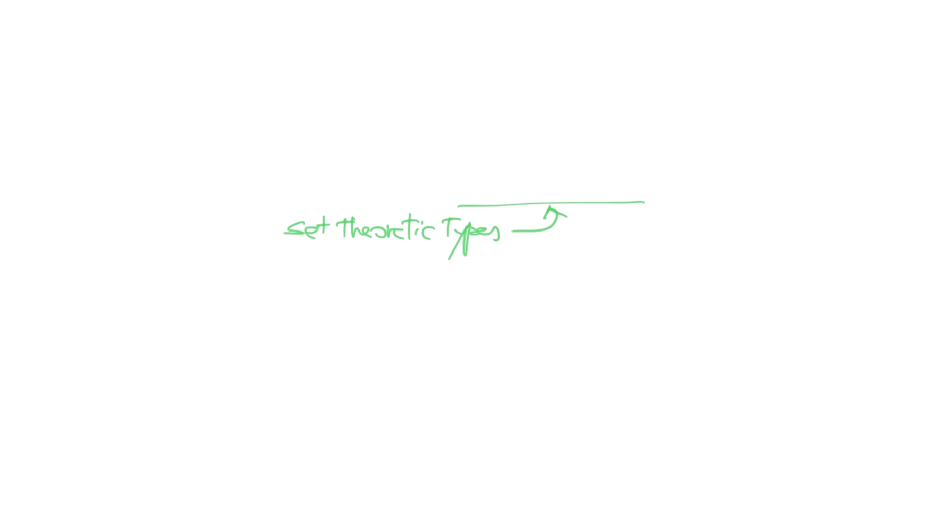
\includegraphics[scale=1]{images/hw-settheore.pdf}\end{textblock}}%
\only<3>{\begin{textblock}{5}(0,0)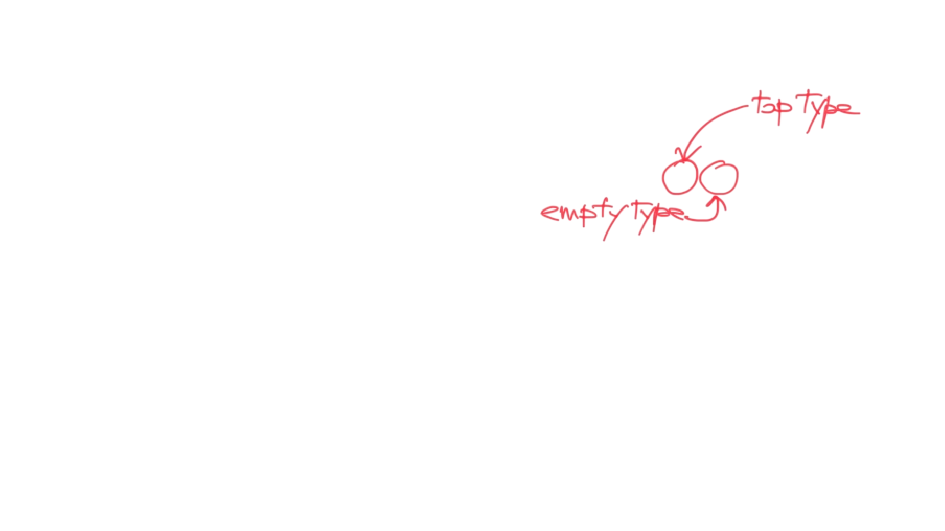
\includegraphics[scale=1]{images/hw-topbottom.pdf}\end{textblock}}%
\pause[4]%
\medskip
\textbf{\color{darkslateblue}The values that match a pattern $p$ form a type}:
\centerline{\color{magenta}
$\accept{p} = \{ v\mid v\text{ is a value that matches }p\}
$}

\textbf{\color{darkslateblue}(the accepted type of pattern $p$)}, e.g., $\Bl\accept{\patpair{x}{y}}=\pair\Any\Any$, the type of all pairs.
\end{frame}



\begin{frame}
\frametitle{3. Precise typing of pattern matching (II)}\xdef\matchframenumber{\insertframenumber}\transdissolve<4>% \matchframenumber is referenced in core.tex

\textbf{\color{darkslateblue}Boolean type connectives are needed to type pattern matching:}

\smallskip

    \hspace*{5mm}{\Bl$\texttt{ match }  e  \texttt{ with } p_1 \texttt{ -> } e_1 \texttt{ | } p_2\texttt{ -> } e_2$}

   \smallskip

Suppose that $\Bl e:\T$\vspace{2mm}
{\setlength{\leftmargini}{0.75em}\setlength{\labelsep}{0.3em}%
\begin{itemize}\setlength{\topsep}{3.5mm}\setlength{\itemsep}{0.2mm}
\item To infer the type $\Bl\T_1$ of $\Bl e_1$ we need {\color{blue}$\T\And \accept{p_1}$};
\item To infer the type $\Bl\T_2$ of $\Bl e_2$ we need {\color{blue}$(\T\setminus \accept{p_1})\And \accept{p_2}$;}\hfill{\textcolor{gray}{\small($\texttt{S}\setminus\T = \texttt{S}\!{\And}\!\neg{\T}$: negation)}}
\pause
\item The type of the match expression is {\color{blue}$\T_1\Or \T_2$}.
\item Pattern matching is exhaustive if $\color{blue}\T\leq\accept{p_1}\Or \accept{p_2}$.
\end{itemize}}
\vspace{-1mm}
\pause
\textbf{Formally:}
\vspace{-2mm}
\begin{mathpar}\Bl
\infer[{[Match]}]
{\Gamma\vdash e:\T\and\Gamma, \T\!\!\And\!\!\accept{p_1\!}/p_1\vdash e_1:\T_1\and \Gamma, \T\setminus\accept{p_1\!}/p_2\vdash e_2:\T_2}
{\Gamma\vdash \texttt{match } e \texttt{ with }p_1 \texttt{->} e_1 \texttt{ | }p_2 \texttt{->} e_2 : \T_1\Or\T_2 }\mbox{\small($\T\leq\accept{p_1\!}\Or\accept{\!p_2\!}$)}
\end{mathpar}
\vspace{-4mm}

\small\color{gray}
where $\Bl \T/p$ is the type for the capture variables in $\Bl p$ when it is matched against values in $\Bl \T$.

\only<4>{\begin{textblock}{5}(0,0)
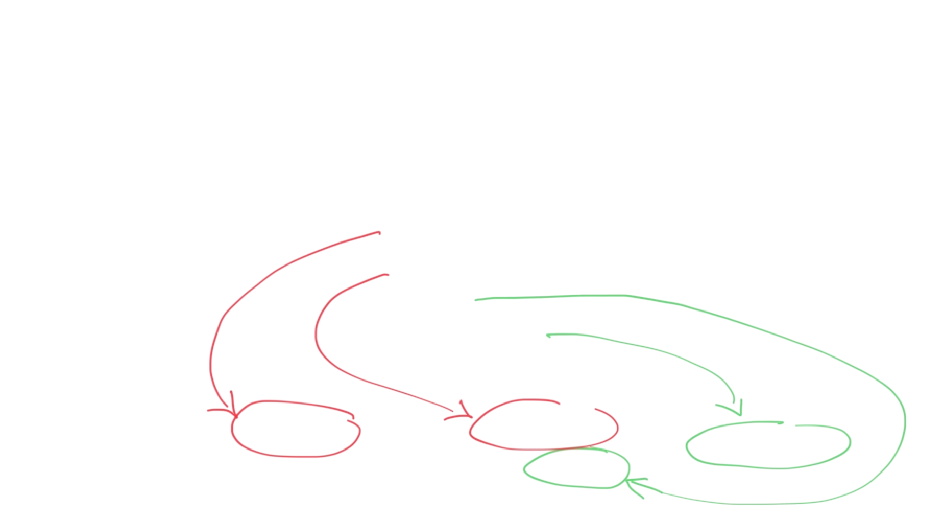
\includegraphics[scale=1]{images/hw-caseexp.pdf}
\end{textblock}}
\end{frame}

\subsection{Semantic subtyping}
\begin{frame}
\frametitle{Semantic subtyping}\vspace{-4mm}

Union and intersection types are now common (TypeScript, Python, Scala 3, Ceylon, \ldots);
negation types are rare.

\smallskip
\textbf{\color{darkslateblue}Our approach: \emph{semantic subtyping}, i.e., subtyping defined by what types mean.}

\smallskip
\begin{columns}[T,onlytextwidth]
  \begin{column}{0.58\textwidth}
    \begin{block}{How does it work?}
      \begin{enumerate}\setlength{\itemsep}{1pt}
        \item Types denote sets of values: $\sem{t}$
        \item Connectives are set operations:\\
              $\sem{t\vee s}=\sem{t}\cup\sem{s}\quad\sem{t\wedge s}=\sem{t}\cap\sem{s}$\\
              $\sem{\neg t}=\sem{t}^{\complement}$
        \item Subtyping is inclusion:\quad $t\leq s \iff \sem{t}\subseteq\sem{s}$
        \item Derive algorithms to decide $\leq$ and compute type operators
      \end{enumerate}
    \end{block}
  \end{column}
  \begin{column}{0.39\textwidth}
    \begin{block}{Why not subtyping rules?}
      Rule-based systems end up incomplete and fragile: e.g.,\\[1mm]
      \centerline{$(\Int\vee\Bool)\times\Int\ \leq$}
      \centerline{$(\Int\times\Int)\vee(\Bool\times\Int)$}\vspace{1mm}
      may not be derivable.

      \smallskip
      With semantic subtyping, all set-theoretic laws hold for \textbf{free}.
    \end{block}
  \end{column}
\end{columns}

\end{frame}



\section{Elixir basic typing}

\begin{frame}
\frametitle{Outline} 
\tableofcontents[currentsection]
\end{frame}

\begin{frame}
\frametitle{Putting the theory to work: Elixir}\vspace{-3mm}
\begin{block}{The language}
\begin{itemize}
\item Dynamic and functional, Ruby-like syntax, strong emphasis on metaprogramming
\item Runs on the Erlang VM: distributed and fault-tolerant applications
\item Rich ecosystem of libraries and frameworks, nearly 100K developers
\item In production at Apple, Discord, PepsiCo, BBC, Adobe, Spotify, \ldots
\end{itemize}
\end{block}

\begin{block}{The type system}
\begin{itemize}
\item Since 2021, in collaboration with José Valim (creator of Elixir) and the Dashbit team
\item Based on our set-theoretic types: in the compiler since v1.17 (June 2024),\\
      covers the whole language since v1.20 (current version: 1.20.4, August 2026)
\end{itemize}
\end{block}
\end{frame}


\subsection{Simple function types}


\begin{frame}[fragile]
\frametitle{Static Typing 101}
\begin{block}{A function that always errors}
\begin{minted}[escapeinside=!!]{elixir}
def negate(x) when is_integer(x), do: not x
\end{minted}
\end{block}\pause
\begin{block}{Type error message}
\begin{minted}[escapeinside=!!]{elixir}
Type error:
  |  def negate(x) when is_integer(x), do: not x
                                           ^^^^^
        the operator not expects boolean() as arguments,
        but the argument is integer()
\end{minted}
\end{block}
\end{frame}



% \defverbatim[colored]{\intToInt}{
% \begin{minted}{elixir}
% !\spec! !\po!integer() !\arr! integer()!\pc!
% \end{minted}
% }
\defverbatim[colored]{\intToInt}{
\begin{coloredverbatim}
$ (integer() -> integer())
\end{coloredverbatim}
}
\defverbatim[colored]{\negateInt}{
\begin{minted}{elixir}
def negate(x) when is_integer(x), do: -x
\end{minted}
}

\begin{frame}[fragile]
\frametitle{Types as contracts between functions.}
\pause
\begin{block}{Function A: Negate}
\visible<3->{%
\intToInt
}
\vspace{-2mm}
\visible<2->{%
\negateInt
}
\vspace{-1.8mm}
\end{block}
\pause\pause
\begin{block}{Function B: Subtract}
\vspace{-1mm}
\begin{coloredverbatim}
$ (integer(), integer() -> integer())
\end{coloredverbatim}
\vspace{-2mm}
\begin{minted}[escapeinside=!!]{elixir}
def subtract(a, b) when is_integer(a) and is_integer(b) do
    a + negate(b)
end
\end{minted}
\end{block}
\pause
\begin{block}{Question}
\begin{itemize}
    \item What if we modify the implementation of \code{negate}?
\end{itemize}
\end{block}
% \begin{block}{Answer}
% If the implementation of \code{negate} changes and violates the type contract, it could lead to unexpected behavior or errors in the \code{subtract} function. Ensuring that the contract is maintained helps guarantee the correctness of our code.
% \end{block}
\end{frame}

\defverbatim[colored]{\intBool}{
\begin{coloredverbatim}
$ (integer() \oor boolean()) -> (integer() \oor boolean())
\end{coloredverbatim}
}
\defverbatim[colored]{\negateBool}{
\begin{minted}{elixir}
def negate(x) when is_boolean(x), do: not x
\end{minted}
}



\subsection{Unions, intersections, negations}

\begin{frame}[fragile]{Union types: correct, but not precise enough.}
\vspace{-2mm}
\begin{block}{Adding a clause for booleans}
\visible<2->{%
\intBool
}
\vspace{-2.1mm}
\visible<1->{%
\negateInt
\vspace{-2.1mm}
\negateBool
}
\vspace{-2.2mm}
\end{block}
\pause\pause

\vspace{-4mm}

\begin{block}{\vspace{-5mm}}
\vspace{-0.2mm}
\begin{coloredverbatim}
$ (integer(), integer() -> integer())
\end{coloredverbatim}
\vspace{-2.1mm}
\begin{minted}[escapeinside=!!]{elixir}
def subtract(a, b) when is_integer(a) and is_integer(b) do
    a + negate(b)
end
\end{minted}
\end{block}
\pause
\begin{block}{Type error in subtract}
\begin{minted}[fontsize=\footnotesize]{elixir}
Type error:
  | def subtract(a, b) when is_integer(a) and is_integer(b) do
  |   a + negate(b)
        ^ the operator + expects integer(), integer() as arguments,
          but the second argument can be integer() or boolean()
\end{minted}
\end{block}
\end{frame}
% todo: add notes with pdfpc
% \begin{block}{Explanation}
% The `+` operator expects two integer arguments, but the second argument can now be an integer \emph{or} a boolean due to the changes in the `negate` function. 
% \end{block}
\defverbatim[colored]{\intersection}{
\begin{coloredverbatim}
$ (integer()->integer()) \oand (boolean()->boolean())
\end{coloredverbatim}
}
\defverbatim[colored]{\intersectionHalf}{
\begin{coloredverbatim}
$ (integer()->integer()) \oand
\end{coloredverbatim}
}
\defverbatim[colored]{\negateIntBool}{
\begin{minted}[escapeinside=!!]{elixir}
def negate(x) when is_integer(x), do: -x
def negate(x) when is_boolean(x), do: not x
\end{minted}
}

\defverbatim[colored]{\intersection}{
\begin{coloredverbatim}
$ (integer()->integer()) \oand (boolean()->boolean())
\end{coloredverbatim}
}
\defverbatim[colored]{\intersectionHalf}{
\begin{coloredverbatim}
$ (integer()->integer()) \oand
\end{coloredverbatim}
}
\defverbatim[colored]{\negateIntBool}{
\begin{minted}[escapeinside=!!]{elixir}
def negate(x) when is_integer(x), do: -x
def negate(x) when is_boolean(x), do: not x
\end{minted}
}


\begin{frame}[fragile]
\frametitle{Type intersections for functions.}
\begin{block}{A more precise annotation}
\vspace{-4.9mm}
\begin{overlayarea}{\textwidth}{.8cm}
% \only<2>{\intersectionHalf}
\only<2->{\intersection}    
\end{overlayarea}
\vspace{.4mm}
% \hfill
% \vspace{1mm}
\negateIntBool
\vspace{-0.7mm}
\end{block}
\pause\pause
\begin{block}{The function \texttt{subtract} type checks}
\vspace{-2mm}
\begin{coloredverbatim}
$ (integer(), integer() -> integer())
\end{coloredverbatim}
\vspace{-2.1mm}
\begin{minted}[escapeinside=!!]{elixir}
def subtract(a, b) when is_integer(a) and is_integer(b) do
    a + negate(b)
end
\end{minted}
\end{block}
\end{frame}

\defverbatim[colored]{\lognegType}{
\begin{coloredverbatim}
$ (false \oor nil -> true) \oand (\onot (false \oor nil) -> false)
\end{coloredverbatim}
}
\defverbatim[colored]{\lognegSingle}{
\begin{coloredverbatim}
$ (false \oor nil -> true) \oand
\end{coloredverbatim}
}

\begin{frame}[fragile]
\frametitle{Singleton and Negation Types}
\begin{block}{Logical negation}%
\vspace{-9mm}
\begin{overlayarea}{\textwidth}{0.5mm}%
    \only<2>{\lognegSingle}
\only<3>{\lognegType}
\end{overlayarea}%
\hfill \vspace{1mm}
\begin{minted}[escapeinside=||]{elixir}
def logical_neg(x) when x == false or x == nil, do: true
def logical_neg(x), do: false
\end{minted}
\end{block}
\pause
\begin{block}{Types}
\begin{itemize}
    \item Singleton types are types containing exactly one value
    \visible<3->{\item Negation types contain any value that is \emph{not} in the 
    negated type.}
\end{itemize}
\end{block}

\end{frame}

\defverbatim[colored]{\mapSip}{
\begin{coloredverbatim}
$ ([a], (a -> b)) -> [b] \owhen a: term(), b: term()
\end{coloredverbatim}
}
\defverbatim[colored]{\mapSigMinted}{
\begin{minted}{elixir}
!\spec! ([a], (a -> b)) -> [b] !\when! a: term(), b: term()
\end{minted}
}
\defverbatim[colored]{\map}{
\begin{minted}[escapeinside=!!]{elixir}
def map([h | t], fun), do: [fun.(h) | map(t, fun)]
def map([], _fun), do: []
\end{minted}
}


\subsection{Polymorphism}
\begin{frame}[fragile]
\frametitle{Polymorphism with Local Type Inference}

\begin{block}{Expressions and functions can have types containing type variables}
\vspace{-7.2mm}
\begin{overlayarea}{\textwidth}{2mm}
\only<2->{\mapSip}
% \only<2->{\mapSigMinted} 
\end{overlayarea} 
\hfill \vspace{1.4mm}
\visible<1->{\map}
\vspace{-1.5mm}
\end{block}
\pause
\begin{block}{Type Variables}
    \begin{itemize}
        \item Quantified using a postfix \texttt{\color{typeBrique}when} with upper bounds
        % \item First-order polymorphism only
    \end{itemize}
\end{block}
\pause
\begin{block}{System deduces type variable instantiation}
\begin{minted}{elixir}
map([{0, true}], fn {x, y} when is_integer(x) -> x end)
# type [integer()]
\end{minted}
\end{block}
\end{frame}

\defverbatim[colored]{\logorFinal}{
\begin{coloredverbatim}
$ ((false \oor nil, a) -> a) when a: term()
$ (a, term() -> a) when a: \onot(false or nil)
\end{coloredverbatim}
}
\defverbatim[colored]{\logorFirst}{
\begin{coloredverbatim}
$ ((false \oor nil, a) -> a) \oand 

\end{coloredverbatim}
}
\defverbatim[colored]{\logorSecond}{
\begin{coloredverbatim}
$ ((false \oor nil, a) -> a) \oand 
  ((b, term()) -> b) \owhen a: term(), b: \onot(false \oor nil)
\end{coloredverbatim}
}


\begin{frame}[fragile]{Intersection and polymorphism}\transdissolve<4->

\begin{block}{Logical OR}%
\vspace{-7mm}
\begin{overlayarea}{\textwidth}{2mm}
    \only<2>{\logorFirst}
    \only<3->{\logorSecond}
    % \only<4>{\logorFinal}
\end{overlayarea}%
\hfill \break 
\begin{minted}[escapeinside=!!]{elixir}
def logical_or(x, y) when x == false or x == nil, do: y
def logical_or(x, _), do: x
\end{minted}
\end{block}
\pause\pause\pause\pause
\textbf{\color{darkslateblue}Bounded Polymorphism:}
\[\color{typeBrique}\forall (s{\leq}\alpha{\leq} u).t \quad\stackrel{def}{=}\quad (\forall \alpha).t[\alpha:=(s{\vee}(\alpha{\wedge} u))]\]
\only<4>{\begin{textblock}{5}(0,0)
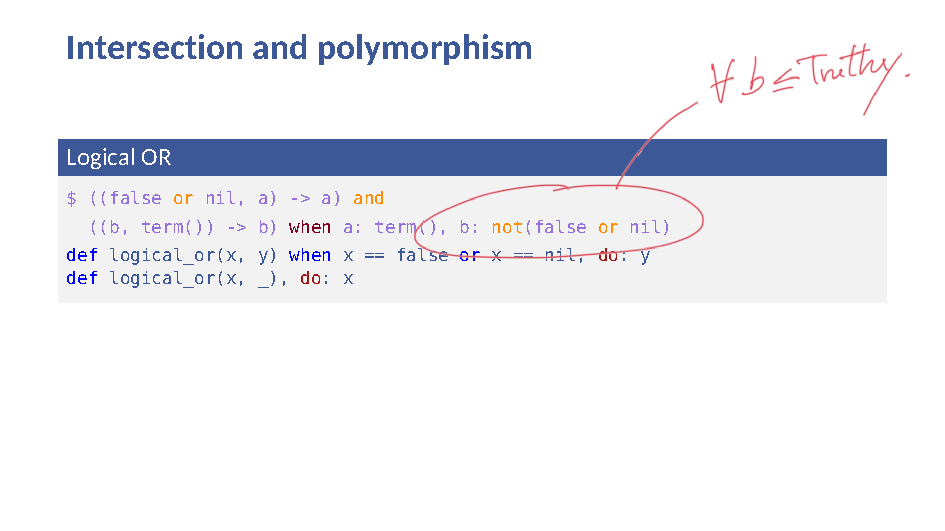
\includegraphics[scale=1]{images/slide-bounded_q.pdf}
\end{textblock}}
\end{frame}





\section{Guard analysis}
\begin{frame}
\frametitle{Outline} 
\tableofcontents[currentsection]
\end{frame}


\subsection{Case expressions: redundancy, exhaustiveness, and narrowing}

\begin{frame}[fragile]
\frametitle{Pattern Matching: Case expressions}
\begin{block}{Using a case expression}
\begin{minted}[escapeinside=!!]{elixir}
def negate(x), do: (case x do
  x when is_integer(x) -> -x
  x when is_boolean(x) -> not x
end)
\end{minted}
\end{block}

\begin{block}{Using multiple function clauses}
\begin{minted}[escapeinside=!!]{elixir}
def negate(x) when is_integer(x), do: -x
def negate(x) when is_boolean(x), do: not x
\end{minted}
\end{block}

\textbf{\color{darkslateblue}Both are equivalent, but the second is preferred in Elixir.}
\end{frame}

\defverbatim[colored]{\result}{
%\vspace{-1.5mm}
\begin{minted}[escapeinside=||,fontsize=\small]{elixir}
|\spec| |\ty| result() = 
    %{output: :ok, socket: socket()} or
    %{output: :error, message: :timeout or {:delay, integer()}}
\end{minted}
\vspace{-1.5mm}
}

\begin{frame}[fragile]
\frametitle{Exhaustiveness and redundancy checking}
\vspace{-7mm}
\begin{block}{\vspace{-5mm}}
\result
\end{block}
\pause

\begin{block}{Exhaustiveness checking: handling all cases}
\begin{minted}[escapeinside=||,fontsize=\small]{elixir}
|\spec| result() -> string()
def handle(r) when r.output == :ok, do: "Msg received"
def handle(r) when r.message == :timeout, do: "Timeout"
\end{minted}
\pause
\vspace{-1.8mm}
\begin{minted}[fontsize=\small]{elixir}
#=> Type Warning: non-exhaustive pattern matching
\end{minted}
\end{block}
\pause

\defverbatim[colored]{\unusedBranch}{
\begin{minted}[fontsize=\small]{elixir}
#=> Type Warning: unused branch
\end{minted}
}

\begin{block}{Redundancy checking: detecting unused clauses}
\begin{minted}[escapeinside=||,fontsize=\small]{elixir}
|\spec| result() -> string()
def handle(r) when r.output == :ok, do: "Msg received"
def handle(r) when r.output == :error, do: "Error raised"
def handle(%{socket: _}), do: "Socket found"
\end{minted}
\pause%
\vspace{-1.6mm}\unusedBranch\vspace{-1.7mm}
\end{block}
\end{frame}

% add a fourth branch for overlapping, by matching 
% on :socket

% remove? no time
\begin{frame}[fragile]
\transdissolve
\frametitle{Narrowing: inferring more precise types}

\vspace{-11mm}%was \vspace{-4mm}
\begin{block}{\vspace{-5mm}}
\result
\end{block}\pause
\begin{block}{Automatically infer a return type}
\begin{minted}[escapeinside=||,fontsize=\footnotesize]{elixir}
|\spec| result() -> _
def handle(r) when r.output == :ok, do: {:accepted, r.socket}
def handle(r) when is_atom(r.message), do: r.message
def handle(r), do: {:retry, elem(r.message, 1)}
\end{minted}
\pause\vspace{-1.7mm}
\begin{minted}[fontsize=\footnotesize]{elixir}
#=> Return type: {:accept, socket()} or :timeout or {:retry, integer()}
\end{minted}
\vspace{-1.2mm}
\end{block}
\pause\pause\pause\pause
\begin{block}{Inferring a more precise type}
\begin{minted}[fontsize=\footnotesize,escapeinside=||]{elixir}
|\spec| (%{output: :ok, socket: socket()} -> {:accept,socket()}) and
  (%{output: :error, message: :timeout} -> :timeout) and
  (%{output: :error, message: {:delay,integer()}} -> {:retry,integer()})
\end{minted}
\end{block}
\only<4>{\begin{textblock}{5}(0,0)
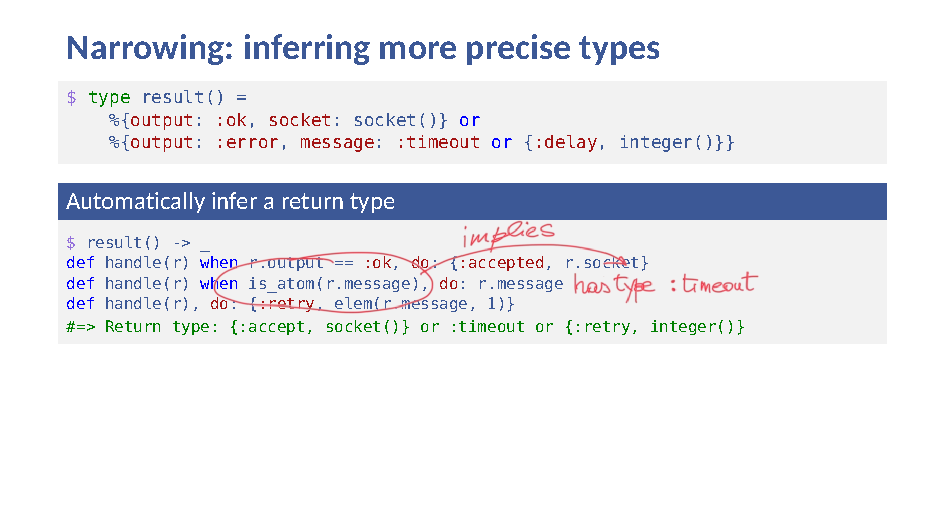
\includegraphics[scale=1]{images/slide-narrow1.pdf}
\end{textblock}}

\only<5>{\begin{textblock}{5}(0,0)
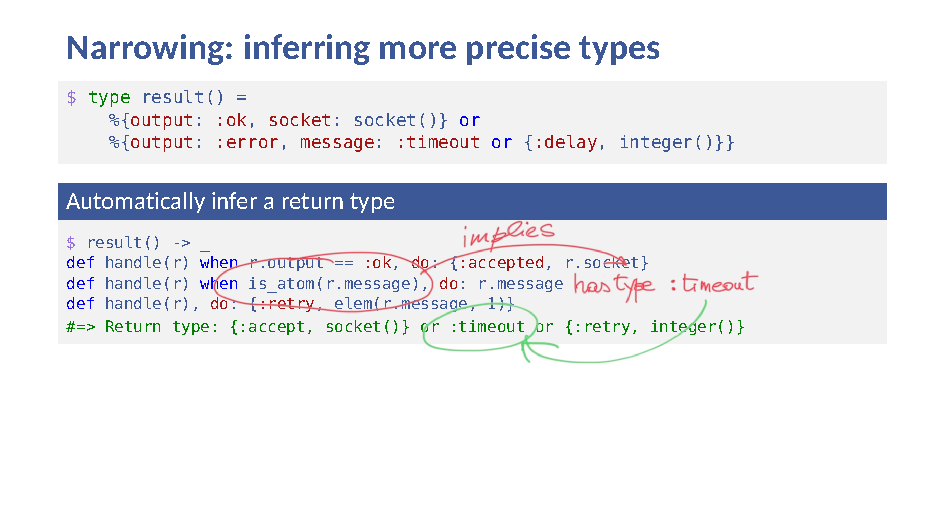
\includegraphics[scale=1]{images/slide-narrow2.pdf}
\end{textblock}}
\only<6>{\begin{textblock}{5}(0,0)
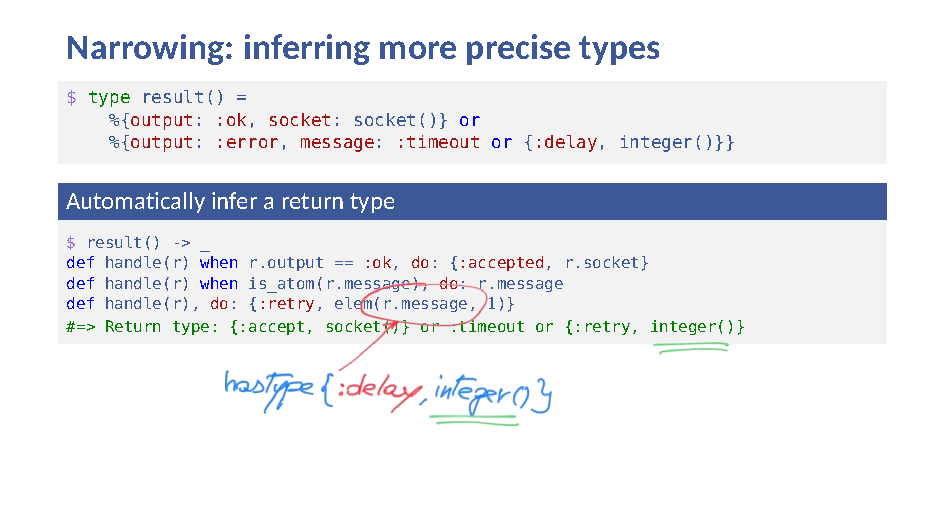
\includegraphics[scale=1]{images/slide-narrow3.pdf}
\end{textblock}}

\only<8>{\begin{textblock}{5}(0,0)
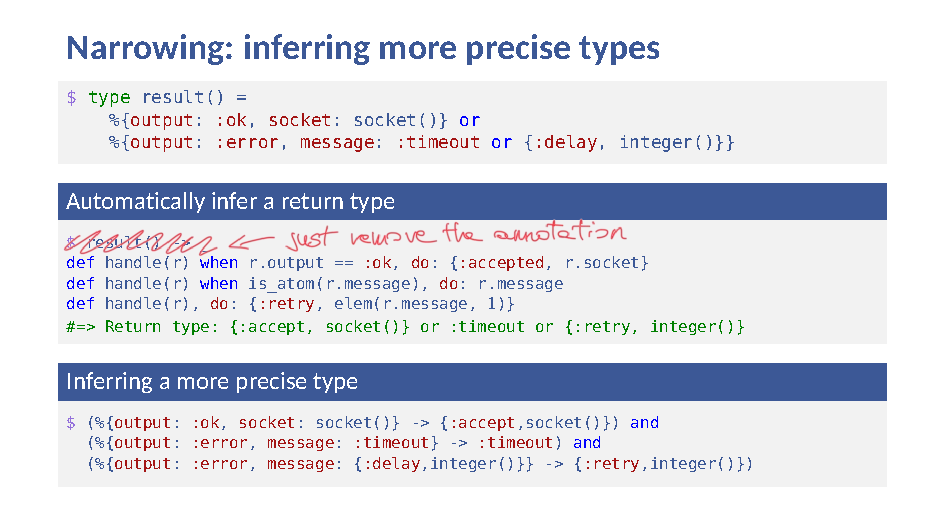
\includegraphics[scale=1]{images/slideNarrowing.pdf}
\end{textblock}}
\end{frame}



\section{Gradual typing}

\begin{frame}
\frametitle{Outline} 
\tableofcontents[currentsection]
\end{frame}

\begin{frame}
\frametitle{Gradual typing: no big-bang migration}
\textbf{\color{darkslateblue}Two non-negotiable requirements for real-world adoption by existing languages:}\\
\textbf{\hspace*{.4mm}1.} You do not have to type-annotate your entire codebase at once.\\
\textbf{2.} Types do not modify the run-time semantics of existing programs.

\medskip

\begin{block}{The \code{dynamic()} type}
\begin{itemize}
\setlength{\itemsep}{-0pt}
\item May turn into any other type at runtime: typed and untyped code coexist
      seamlessly
\item Offers a more relaxed type safety guarantee:\\
 If some program \code{e} has type \code{integer()} and evaluates to a value, \\
      then this value is of type \code{integer()}.
\end{itemize}
\end{block}

\end{frame}
%%% def boolean_id(x), do: x
\defverbatim[colored]{\weakApp}{
\begin{minted}{elixir}
id_weak(x_dyn)                    !\textcolor{gray}{\footnotesize x\textunderscore{}dyn may be a string, and}!
# type dynamic()                  !\textcolor{gray}{\footnotesize id\textunderscore{}weak returns it unchanged}!
\end{minted}
}
\defverbatim[colored]{\strongApp}{
\begin{minted}{elixir}
id_weak(x_dyn)                    id_strong(x_dyn)
# type dynamic()                  # type integer() 
\end{minted}
}
\defverbatim[colored]{\strongAppPropagation}{
\begin{minted}{elixir}
id_weak(x_dyn)                    id_strong(x_dyn)
# type dynamic()                  # type integer() !\color{magenta}and dynamic()!
\end{minted}
}

\begin{frame}
\frametitle{The gradual typing conundrum}
\textbf{\color{darkslateblue}Typing every expression by \code{dynamic()} is trivially sound \ldots but hardly useful.}

\bigskip
\pause
The system must fulfill two opposite requirements
\begin{enumerate}
	\item it must use \code{dynamic()}  as little as possible so as to be useful, and
	\item it must use \code{dynamic()} enough so as not to hinder the versatility of
	      gradual typing
\end{enumerate}


\bigskip
\pause
The first requirement is fulfilled by the typing of \textbf{\color{darkslateblue}strong functions}, which leverage the run-time checks written by the programmer, or performed by the VM\\[3mm]
The second requirement is fulfilled by the \textbf{\color{darkslateblue}propagation of \code{dynamic()}}.
\end{frame}

\subsection{Strong function types}

\begin{frame}[fragile]{Strong function types}\transdissolve<2,4->
\vspace{-1.5mm}
\begin{block}{(Weak) function type}
\begin{minted}[escapeinside=!!]{elixir}
!\spec! integer() -> integer()
def id_weak(x), do: x !\label{c1}!
\end{minted}
\end{block}
\vspace{-1.6mm}
\pause
\begin{block}{Let \code{x_dyn} be of type \code{dynamic()}}
\vspace{-4.9mm}
    \begin{overlayarea}{\textwidth}{1.3cm}
        \only<2-3>{\weakApp}
        \only<4-7>{\strongApp}
        \only<8->{\strongAppPropagation}
   \end{overlayarea}
\end{block}
\vspace{-1.5mm}
\pause
\begin{block}{Strong function type \only<6->{\smash{(by the programmer)}}}
\begin{minted}[linenos=false,escapeinside=!!]{elixir}
!\spec! integer() -> integer()
def id_strong(x) when is_integer(x), do: x 
\end{minted}
\end{block}
% \begin{block}{Application}
% \begin{minted}{elixir}
% !\spec! dynamic() -> {dynamic(), integer()}
% def dynamic_fun(x), do: {id_weak(x), id_strong(x)}
% \end{minted}
% \end{block}
\pause\pause\pause\pause
\vspace{-.5mm}
% \frametitle{Strong function types (by the VM)}
\begin{block}{Strong function type (by the VM)}
\begin{minted}[linenos=false,escapeinside=!!]{elixir}
!\spec! number() -> number()
def double(x), do: x + x
\end{minted}
\end{block}
% \begin{itemize}
% \item Functions with strong types guarantee correct output or runtime type-check failure
% \item Ensures stronger type safety guarantee without modifying Elixir compilation
% % \item Take into account user type checks
% % \item Allows for propagation of \code{dynamic()} type in certain cases
% \end{itemize}
\only<5,6>{\begin{textblock}{15}(1.3,12.9)
    \textbf{\color{darkslateblue}\large Strong function: on \emph{any} argument, even outside its domain, it returns a result in its codomain or fails}
\end{textblock}}
\only<9>{\begin{textblock}{5}(0,0)
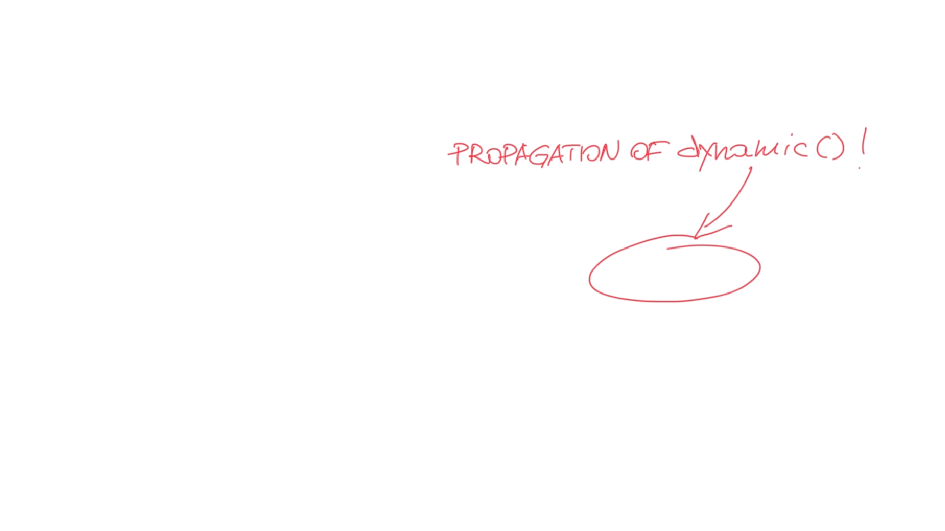
\includegraphics[scale=1]{images/hw-dynprop.pdf}
\end{textblock}}
\end{frame}




\defverbatim[colored]{\dynType}{
\begin{minted}{elixir}
#=> negate(x_dyn): (integer() or boolean()) !\color{magenta}and dynamic()!
\end{minted}
}
\defverbatim[colored]{\wrongType}{
\begin{minted}{elixir}
#=> negate(x_dyn): (integer() or boolean())
\end{minted}
}
\defverbatim[colored]{\typeError}{
\begin{minted}{elixir}
#=> Without propagation: type error, + undefined for booleans
\end{minted}
}
\defverbatim[colored]{\goodType}{
\begin{minted}{elixir}
#=> subtract: (dynamic(), dynamic() -> number())
\end{minted}
}
\defverbatim[colored]{\betterType}{
\begin{minted}{elixir}
#=> subtract: (dynamic(), dynamic() -> number() !\color{magenta}and dynamic()!)
\end{minted}
}
\defverbatim[colored]{\subtract}{
\begin{minted}{elixir}
def subtract(a, b), do: a + negate(b)
\end{minted}
}
\defverbatim[colored]{\subtractann}{
\begin{minted}{elixir}
def subtract(a, b), do: a + negate(b)    !\textcolor{gray}{\footnotesize\char35{} a, b not annotated, hence dynamic()}!
\end{minted}
}

\subsection{Propagation of \texttt{dynamic()}}

\begin{frame}[fragile]{Propagation of \texttt{dynamic()}}\transdissolve<6>
\textbf{\color{darkslateblue}Apply the (strong function) \code{negate()} function to a \code{dynamic()} argument: \code{x_dyn}}
\vspace{-4mm}
\begin{block}{\vspace{-5mm}}
\begin{minted}{elixir}
!\spec! (integer() -> integer()) and (boolean() -> boolean())
def negate(x) when is_integer(x), do: -x
def negate(x) when is_boolean(x), do: not x
\end{minted}
\vspace{-6.1mm}
\begin{overlayarea}{\textwidth}{2mm}
    \only<2-5>{\wrongType}
    \only<6->{\dynType}
\end{overlayarea}
\hfill
\vspace{0.5mm}
\hfill
\end{block}
\pause\pause\vspace{-6mm}
\begin{block}{\vspace{-6mm}}\vspace{-2mm}
\begin{overlayarea}{\textwidth}{9mm}
\only<3>{\subtract}
\only<4->{\subtractann}
\end{overlayarea}
\vspace{-6.5mm}
\begin{overlayarea}{\textwidth}{2mm}
    \only<5>{\typeError}
    \only<7>{\goodType}
    \only<8->{\betterType}
\end{overlayarea}
\hfill
\vspace{0.5mm}
\end{block}
\pause\pause\pause\pause\pause\pause\vspace{-7mm}
\begin{block}{\vspace{-5mm}}
\begin{minted}{elixir}
def concat(a, b), do: a <> negate(b)
\end{minted}
\vspace{-1mm}
\begin{warnverbatim}
\warn incompatible types in binary construction: <<..., negate(b)::binary>>
got type: dynamic(boolean() or integer()), expected type: binary()
\textcolor{gray}{(dynamic(t) is how Elixir prints t and dynamic())}
\end{warnverbatim}
\vspace{-1mm}
\end{block}
\pause
{\small\textbf{\color{darkslateblue}\code{t and dynamic()} is accepted where \code{s} is expected iff \code{t and s} is not \code{none()}}:
\code{dynamic()} is forced to materialize into \code{s}, and is propagated to the result.\par}
\end{frame}


\section{Integration in Elixir}

\begin{frame}
\frametitle{Outline}
\tableofcontents[currentsection]
\end{frame}

\begin{frame}[fragile]
\frametitle{Elixir 1.20: typing without annotations}\vspace{-4mm}
\begin{itemize}\setlength{\itemsep}{0pt}
\item No annotation, no syntactic change: every parameter is typed \code{dynamic()}
\item Types are refined by patterns and guards (guard analysis, Section~3)
\item Inferred types are checked by gradual typing (Section~4)
\item Multi-clause functions get intersection types from their guards (Section~3),
      with \code{dynamic()} propagated to the results (Section~4); for \code{negate}:
\end{itemize}
\vspace{-1mm}
\begin{block}{\vspace{-5mm}}
\begin{coloredverbatim}
(integer() -> integer() \oand dynamic()) \oand
(boolean() -> boolean() \oand dynamic())
\end{coloredverbatim}
\vspace{-1mm}
\end{block}
\vspace{-2.5mm}
\begin{block}{The error is still caught}
\begin{minted}[fontsize=\footnotesize]{elixir}
def bad(b) when is_boolean(b), do: 1 + negate(b)
\end{minted}
\vspace{-1mm}
\begin{warnverbatim}
\warn incompatible types given to Kernel.+/2: 1 + negate(b)
given types: integer(), dynamic(boolean())   \textcolor{gray}{(i.e., boolean() and dynamic())}
\end{warnverbatim}
\vspace{-1mm}
\end{block}
\pause
{\small\textbf{\color{darkslateblue}Type signatures} (the \texttt{\$} of this talk) are planned, after
efficient recursive and parametric types (the polymorphism of Section~2), map traversal,
and typed structs.\par}
\end{frame}

\begin{frame}
\frametitle{Status of the integration}\vspace{-4mm}
\begin{itemize}\setlength{\itemsep}{0pt}
\item v1.17 (June 2024): gradual set-theoretic types for atoms, maps, basic types
\item v1.18: type-checked function calls, inference for patterns and return types
\item v1.19 (Oct.\ 2025): all constructs; function types; \textit{protocols} (\`a la type classes)
\item \textbf{v1.20 (June 2026, now 1.20.4): typing covers the whole language}: full guard analysis, intersection types inferred for multi-clause functions
\end{itemize}
\end{frame}

% Empirical results for Guillaume's part; timing table moved to a chart.
% Guillaume's empirical-evaluation segment (about 5--6 minutes).
% Source: core-elixir/core-elixir-paper, revision 44493a5, inspected 2026-10-05.
% Keep the corpus experiments separate from the Elixir v1.19 timing snapshot.
% All charts are native TikZ objects; the measurements remain editable here.
\newcommand{\perfsource}[1]{%
  \vfill
  {\scriptsize\color{gray}Source: Castagna \& Duboc, Core Elixir paper. #1\par}}

\begin{frame}[t,label=perf-corpus]
\frametitle{Precision on real Elixir code}
\textbf{17 open-source projects, without user type annotations}

\bigskip
\begin{columns}[T,onlytextwidth]
  \begin{column}{0.47\textwidth}
    {\fontsize{34}{38}\selectfont\bfseries\color{darkslateblue}86.1\%\par}
    \smallskip
    \textbf{Exact pattern/guard pairs}\par
    \smallskip
    {\small 141,755 of 164,701 analyzed pairs\par}
    \medskip
    The analysis identifies exactly which inputs match.
  \end{column}
  \begin{column}{0.47\textwidth}
    {\fontsize{34}{38}\selectfont\bfseries\color{darkslateblue}61.7\%\par}
    \smallskip
    \textbf{Informative inferred returns}\par
    \smallskip
    {\small 43,158 of 69,976 inferred arrows\par}
    \medskip
    The return type differs from\par
    \code{dynamic()}. For example,\par
    \code{dynamic(integer())}.
  \end{column}
\end{columns}

\perfsource{Empirical evaluation and compilation measurements.}
\note{Source: evaluation.tex, lines 85--114 and 182--257; main.tex,
  appendix Guard Exactness Corpus, lines 4760--4799. Both displayed ratios
  are weighted counts over the selected 17-project corpus. Do not confuse
  the 86.07 percent aggregate with the separate six-codebase measurement
  of 64.44 percent. Exactness counts analyzed pattern/guard pairs, not
  functions or bugs. Postgrex is an outlier at 34.83 percent, largely because
  generated list-head dispatch patterns are conservatively treated as inexact.
  Return informativeness counts arrows, not functions. The return experiment
  covers 517,999 lines of code. A return gets score 1 whenever it is not
  exactly dynamic(); this is a coarse binary measure, not a percentage of
  fully statically typed code. Inference does not use inferred function types
  across module boundaries in this experiment, which limits return information.
  Reproduction artifacts: https://github.com/gldubc/core-elixir-experiments.}
\end{frame}

\begin{frame}[fragile,t,label=perf-narrowing]
\frametitle{Narrowing through a nested condition}
\textbf{Elixir adaptation of \textit{If-T}: 12/13 core items pass}
\hfill{\small Research compiler}

\bigskip
\begin{columns}[T,onlytextwidth]
  \begin{column}{0.61\textwidth}
\begin{minted}[fontsize=\small]{elixir}
# x, y : term()
if if(is_integer(x),
      do: is_binary(y),
      else: false) do
  x + byte_size(y)
else
  0
end
\end{minted}
  \end{column}
  \begin{column}{0.34\textwidth}
    \textbf{Inside the outer branch}
    \medskip
    \code{x : integer()}\par
    \code{y : binary()}\par
    \medskip
    {\small The outer condition can only be true when \emph{both} tests
    succeed.\par}
    \smallskip
    \textbf{Elixir accepts the program.}
  \end{column}
\end{columns}

\medskip
\textbf{Paper snapshot: 7 of 11 other implementations miss this item.}\par
{\small TypeScript, Flow, mypy, Pyright, Luau, \textsf{ty}, Pyrefly.\par}
\note{Source: evaluation.tex, lines 119--180, and main.tex, appendix
  If-T Benchmark Reproduction, lines 4731--4758. This is the Elixir adaptation
  of the 13 core items, using the research branch with asserted function
  annotations. It is not a claim that upstream Elixir supports those
  annotations, nor a direct cross-language ranking. The code shown is the
  body of the positive \texttt{nesting\_condition} example, from
  ifT-benchmark/Elixir/main.ex, lines 251--273. The full benchmark asserts
  (term(), term() -> integer()) on f/2. Preserve the nested conditional:
  rewriting it as an and-test would change the point of the example.
  The outer true branch requires both x to be an integer and y to be a binary.
  In the rejected variant, replace the inner else: false with
  else: is\_binary(y). Now y can be a binary while x is not an integer,
  so the addition is unsafe. Elixir rejects that variant.
  The paper's table and results-core.md record misses for TypeScript, Flow,
  mypy, Pyright, Luau, ty, and Pyrefly; passes for Elixir, Typed Racket,
  Sorbet, MLsem, and Typed Clojure. A miss means at least one expectation
  fails, not necessarily that an invalid program was accepted.
  This is a recorded benchmark snapshot, not a statement about latest versions.
  Archived benchmark revision: e25b30a529d5196d8cf01e3fe6b1b5a9cd88b744.
  Archived research compiler: 3684a541ed2ce9f83cd74fd46a7bae69081f017b.
  All negative witnesses across the core items are rejected. The only core
  miss remains alias, where a saved Boolean fails to refine the tested value.
  Reference: Guo and Greenman, If-T: A
  Benchmark for Type Narrowing, Programming 10(2), article 17, 2025.
  Reproduction artifacts: https://github.com/gldubc/core-elixir-experiments.}
\end{frame}

\begin{frame}[t,label=perf-propagation]
\frametitle{Removing dynamic propagation}
\textbf{Compile the same 17 projects with and without propagation}

\bigskip
\begin{columns}[c,onlytextwidth]
  \begin{column}{0.66\textwidth}
    \begin{tikzpicture}[x=0.027cm,y=1cm]
      \node[anchor=east,font=\small] at (-5,1.1) {Full checker};
      \node[anchor=east,font=\small,align=right] at (-5,0) {Without dynamic\\propagation};
      \fill[darkslateblue] (0,0.88) rectangle (94,1.32);
      \fill[darkslateblue] (0,-0.22) rectangle (94,0.22);
      \fill[typeOrange] (94,-0.22) rectangle (158,0.22);
      \node[anchor=west,font=\small\bfseries] at (97,1.1) {94};
      \node[anchor=west,font=\small\bfseries] at (161,0) {158};
      \draw[gray!65] (0,-0.65) -- (160,-0.65);
      \foreach \n in {0,80,160} {
        \draw[gray!65] (\n,-0.65) -- (\n,-0.72);
        \node[anchor=north,font=\scriptsize,text=gray] at (\n,-0.76) {\n};
      }
      \node[anchor=north,font=\small] at (80,-1.12) {Project type warnings};
    \end{tikzpicture}
  \end{column}
  \begin{column}{0.29\textwidth}
    {\fontsize{32}{36}\selectfont\bfseries\color{typeOrange}+64\par}
    \smallskip
    \textbf{additional warnings}\par
    \medskip
    {\small Six projects are unchanged.\par}
  \end{column}
\end{columns}

\medskip
{\small Dynamic propagation avoids requiring extra checks on results of
function calls in existing code.\par}

\note{Source: evaluation.tex, lines 260--333, table \texttt{dynamic\_propagation\_removal}.
  Full checker: 94 project type warnings. Static variant: 158. Difference:
  64, or approximately 68 percent. Warnings from dependencies are excluded.
  The paper's static variant suppresses the dynamic component propagated
  through strong applications, replacing t and dynamic() with t. These are
  warning counts, not a validated count of additional bugs or false positives.
  The six unchanged projects are HexPm, Ecto, Phoenix, MixSBOM, Nerves, and
  AbsintheFederation. For example, using a returned integer-or-Boolean in
  addition may require an explicit \texttt{is\_integer} check without propagation.
  Reproduction artifacts: https://github.com/gldubc/core-elixir-experiments.}
\end{frame}

\begin{frame}[t,label=perf-cost]
\frametitle{Compilation cost on production code}
\textbf{Checking as a share of total compilation time, Elixir v1.19}

\bigskip
\begin{columns}[c,onlytextwidth]
  \begin{column}{0.62\textwidth}
    \begin{tikzpicture}[x=0.51cm,y=0.58cm]
      \foreach \name/\share/\row in {Credo/2.4/4,Livebook/3.3/3,Hex/5.3/2,Phoenix/6.3/1,Remote/8.5/0} {
        \node[anchor=east,font=\small] at (-0.2,\row) {\name};
        \fill[darkslateblue] (0,\row-0.22) rectangle (\share,\row+0.22);
        \node[anchor=west,font=\small\bfseries] at (\share+0.12,\row) {\share\%};
      }
      \draw[gray!65] (0,-0.55) -- (10,-0.55);
      \foreach \n in {0,5,10} {
        \draw[gray!65] (\n,-0.55) -- (\n,-0.68);
        \node[anchor=north,font=\scriptsize,text=gray] at (\n,-0.75) {\n\%};
      }
    \end{tikzpicture}
  \end{column}
  \begin{column}{0.33\textwidth}
    \textbf{Remote}\par
    \smallskip
    {\fontsize{30}{34}\selectfont\bfseries\color{darkslateblue}19.5\,s\par}
    \smallskip
    to check \textbf{24,292 modules}\par
    \medskip
    {\small Over 1 million lines of code\par
    228.8\,s total compilation\par}
  \end{column}
\end{columns}

\note{Source: implementation.tex, lines 307--332, v1.19 table. These are
  shares of total compilation, not a controlled estimate of net added overhead.
  Exact checking/total times (seconds): Credo 0.027/1.095; Livebook
  0.102/3.051; Hex 0.065/1.232; Phoenix 0.029/0.461; Remote
  19.476/228.801. Percentages reproduce the paper's reported rounded values.
  Remote's 24,292 modules are counted; its over-one-million LoC is a
  conservative estimate. The timing category includes deprecated-API and
  function-definition checks, some of which replace earlier compiler checks.
  These are the paper's v1.19 measurements, separate from the newer empirical
  corpus experiments. The manuscript does not specify hardware, repeats, or
  variance. Do not use the v1.18/v1.19 snapshots as a controlled speedup
  comparison: the codebases evolved between evaluations.}
\end{frame}


\begin{frame}[fragile]
\frametitle{Status of the integration}\vspace{-3mm}
\begin{itemize}
\item Very positive feedback from developers on versions 1.17 to 1.20
\item No syntactic changes and no annotations required: particularly appreciated
\item Errors found in tested and reviewed code, in production for months or years
\end{itemize}

\medskip\pause

\begin{block}{Real-world Bug Discoveries}
\begin{itemize}
    \setlength{\itemsep}{0pt}
\item \textbf{Phoenix} (deployed on 12,000+ websites): an exception handler reads the \code{message} field, which not every exception defines: the error branch can itself crash
\item \textbf{Remote} (24,000 modules): \code{String.Chars} called on a tuple in a rarely executed error branch, undetected by tests
\item \textbf{Dead code}: 14 fixes, at least 179 lines removed in 9 projects (Postgrex, Flame, LiveView, Ecto, ExDoc, Livebook, Ash, Phoenix, Spitfire)
\item \textbf{v1.20}: porting one company application to 1.20 revealed about 500 problems missed by 1.19, mostly dead code but also real bugs\vspace{-1mm}
\end{itemize}
\end{block}
\end{frame}

\begin{frame}[fragile]
\frametitle{\mbox{Several languages use (more or less) semantic subtyping}}
\hspace*{-0.8em}%
\begin{minipage}{1.06\textwidth}
  \setlength{\leftmargini}{1.9em}
\begin{itemize}\setlength{\itemsep}{2pt}  \setlength{\rightmargin}{-12pt} % reduce right margin (use full width)

  \item \textbf{Elixir} — in the compiler since v1.17 (2024), whole
        language since v1.20 (2026)
        % (Discord, Pinterest,PepsiCo, \ldots)

  \item \textbf{Python (\textsf{ty})} — Astral's high-performance type
        checker reuses data-structures and optimisations developed for
        Elixir, and is migrating to a full semantic subtyping implementation.

  \item \textbf{Ballerina} (WSO2) — uses semantic subtyping since its
        Swan Lake release

  \item \textbf{Luau} (Roblox) — falls back to semantic subtyping when
        syntactic subtyping is insufficient

  \item \textbf{Erlang} — \emph{RPTU} (Kaiserslautern) develops \textsl{Ethylizer} which reconstructs set-theoretic types  for unannotated
        code by using our semantic subtyping algorithms and techniques; \\
        \emph{Meta} develops \textsl{eqWAlizer} to type WhatsApp's Erlang codebase, building on our semantic-subtyping-based gradual typing.

  \item \textbf{R} — \emph{U.\ Karlova} (Prague) is developing a type system for R
        based on semantic subtyping

  \item \textbf{Julia} — core developers cite semantic subtyping as
        direct inspiration for Julia's type system

  \item \textbf{CDuce} and its spin-offs SSTT and MLsem — the original
        theoretical proving grounds
\end{itemize}
\end{minipage}
\end{frame}


% Future work: one frame per topic, what fails today (Elixir 1.20.4, checked) and what the
% planned types catch (proposed syntax, not final)
% new syntax (not in Elixir today), in one very visible color
\definecolor{newsyntax}{RGB}{230,60,0}
\newcommand{\newkw}[1]{\textcolor{newsyntax}{\textbf{#1}}}

\begin{frame}[fragile]
\frametitle{Future work: typing modules}\vspace{-3mm}
\begin{block}{Today (Elixir 1.20): the type \code{module()} says nothing}
\begin{minted}[fontsize=\footnotesize]{elixir}
defmodule Counter do
  @behaviour GenServer
  def init(:ok), do: {:ok, %{}}
  def handle_call({:bump, k}, _from, s), do: ...
end
GenServer.start_link(Counter, :not_ok)    # no warning: crashes at run time
\end{minted}
\vspace{-1mm}
\end{block}
\pause
\vspace{-2mm}
\begin{exampleblock}{Tomorrow: typed behaviours}
\begin{minted}[fontsize=\footnotesize,escapeinside=||]{elixir}
defmodule Counter do
  |\newkw{\$behaviour}| GenServer|\newkw{[}|init_arg: :ok, call_msg: {:bump, atom()}, reply: integer()|\newkw{]}|
  |\newkw{\$opaque}| state = %{atom() => integer()}
  def init(:ok), do: {:ok, %{}}
  def handle_call({:bump, k}, _from, s), do: ...
end
GenServer.start_link(Counter, :not_ok)    # error: the init_arg of Counter is :ok
\end{minted}
\vspace{-1mm}
\end{exampleblock}
{\small\color{gray}Joint work with A.~Boussaa, A.~Bretagne and J.~Valim; proposed syntax, not final.\par}
\end{frame}

\begin{frame}[fragile]
\frametitle{Future work: typing processes}\vspace{-3mm}
\begin{block}{Today (Elixir 1.20): the type \code{pid()} says nothing}
\begin{minted}[fontsize=\footnotesize]{elixir}
send(self(), true)
receive do y -> IO.puts(y + y) end        # no warning: crashes at run time
\end{minted}
\vspace{-1mm}
\end{block}
\pause
\vspace{-2mm}
\begin{exampleblock}{Tomorrow: \code{pid(t)}, where \code{t} is the type of the messages the process accepts}
\begin{minted}[fontsize=\footnotesize,escapeinside=||]{elixir}
|\newkw{\$interface}| {:add, integer()} or boolean()
spawn(fn ->
  send(self(), true)                      # accepted: boolean() is in the interface
  receive do
    {:add, y} -> y + 1                    # y : integer()
    y -> y + y                            # error: y : boolean()
  end
end)
\end{minted}
\vspace{-1mm}
\end{exampleblock}
{\small\color{gray}Joint work with L.~Padovani (Bologna) and D.~Varacca (\'Evry); later, mailbox types to ensure liveness.\par}
\end{frame}

\begin{frame}[fragile]
\frametitle{Future work: record type comprehensions}\vspace{-3mm}
\begin{block}{Today (Elixir 1.20): the result of \texttt{Map.intersect/2} is \texttt{dynamic()}}
\begin{minted}[fontsize=\footnotesize]{elixir}
m = Map.intersect(%{a: 1, b: "x"}, %{b: :ok, c: 2})
m.a                                       # no warning: crashes at run time
m.b + 1                                   # no warning: crashes at run time
\end{minted}
\vspace{-1mm}
\end{block}
\pause
\vspace{-2mm}
\begin{exampleblock}{Tomorrow: record types defined by comprehension over the keys}
{\small Type of \texttt{Map.intersect/2}: the keys \texttt{k} common to both maps, with their type in the second\par}
\begin{minted}[fontsize=\footnotesize,escapeinside=!!]{elixir}
!\spec! (a, b) -> %{k in keyof(a) and keyof(b) | b[k]} when a: map(), b: map()
m = Map.intersect(%{a: 1, b: "x"}, %{b: :ok, c: 2})   # m : %{b: :ok}
m.a                                       # error: unknown key .a
m.b + 1                                   # error: :ok is not a number
\end{minted}
\vspace{-1mm}
\end{exampleblock}
{\small\color{gray}The same comprehensions type \texttt{Map.take}, \texttt{drop}, \texttt{merge}, \texttt{filter}, \ldots; syntax not final.\par}
\end{frame}

\end{document}

%% ----------------------------------------------------------
%%  SLIDE 10 — Why this is the most promising approach
%% ----------------------------------------------------------
\begin{frame}
\frametitle{A proven approach}

\begin{enumerate}\setlength{\itemsep}{4pt}

  \item \textbf{\color{darkslateblue}Faithful to the semantics.}
    $T_1 \leq T_2$ means exactly $\llbracket T_1\rrbracket \subseteq
    \llbracket T_2\rrbracket$ — no axioms, no approximations.

  \item \textbf{\color{darkslateblue}Designed for dynamic idioms.}
    Overloading, pattern matching, and non-uniform branching are all
    described \emph{naturally}, without awkward workarounds.

  \item \textbf{\color{darkslateblue}Gradual typing.}
    Works incrementally.  No flag day, no forced full rewrite.  Start
    with nothing and add types where they help.

  \item \textbf{\color{darkslateblue}Proven in production.}
    Already integrated in Elixir, Python, Ballerina, Erlang.  Finding
    real bugs in real codebases \emph{today}.

  \item \textbf{\color{darkslateblue}Solid theoretical foundations.}
    Backed by 15+ years of peer-reviewed work (JACM, POPL, ICFP,
    OOPSLA).  

  \item \textbf{\color{darkslateblue}Supports formal certification.}
    Soundness is proved, not just tested — directly relevant to
    regulatory requirements for evidence of software assurance.

\end{enumerate}

\end{frame}


%% ----------------------------------------------------------
%%  SLIDE 11 — Takeaways
%% ----------------------------------------------------------
\begin{frame}
\frametitle{Takeaways} \vspace*{-6mm}

\begin{enumerate}[<+->]\setlength{\itemsep}{6pt}

  \item Dynamic languages need static typing — for correctness, tooling,
        and regulatory confidence.

  \item Traditional type systems were not built for dynamic idioms.
        A new model is needed.

  \item Set-theoretic types with semantic subtyping provide that model:
        \emph{expressive, correct, and well-founded}.

  \item Gradual adoption means no disruption — start typing today,
        incrementally.

  \item Already validated across 8+ languages and real-world production
        codebases.

  \item \textbf{\color{darkslateblue}The theory is solid —and still advancing. The practice is proven. The adoption is growing}

\end{enumerate}

\end{frame}


\appendix
\begingroup
% fibeamer prints a footer even on frames with noframenumbering.
\setbeamertemplate{footline}{}
%% Backup material: keep appendix frames unnumbered.
\begin{frame}[t,noframenumbering,label=perf-propagation]
\frametitle{Removing dynamic propagation}
\textbf{Compile the same 17 projects with and without propagation}

\bigskip
\begin{columns}[c,onlytextwidth]
  \begin{column}{0.66\textwidth}
    \begin{tikzpicture}[x=0.027cm,y=1cm]
      \node[anchor=east,font=\small] at (-5,1.1) {Full checker};
      \node[anchor=east,font=\small,align=right] at (-5,0) {Without dynamic\\propagation};
      \fill[darkslateblue] (0,0.88) rectangle (94,1.32);
      \fill[darkslateblue] (0,-0.22) rectangle (94,0.22);
      \fill[typeOrange] (94,-0.22) rectangle (158,0.22);
      \node[anchor=west,font=\small\bfseries] at (97,1.1) {94};
      \node[anchor=west,font=\small\bfseries] at (161,0) {158};
      \draw[gray!65] (0,-0.65) -- (160,-0.65);
      \foreach \n in {0,80,160} {
        \draw[gray!65] (\n,-0.65) -- (\n,-0.72);
        \node[anchor=north,font=\scriptsize,text=gray] at (\n,-0.76) {\n};
      }
      \node[anchor=north,font=\small] at (80,-1.12) {Project type warnings};
    \end{tikzpicture}
  \end{column}
  \begin{column}{0.29\textwidth}
    {\fontsize{32}{36}\selectfont\bfseries\color{typeOrange}+64\par}
    \smallskip
    \textbf{additional warnings}\par
    \medskip
    {\small Six projects are unchanged.\par}
  \end{column}
\end{columns}

\medskip
{\small Dynamic propagation avoids requiring extra checks on results of
function calls in existing code.\par}

\note{Source: evaluation.tex, lines 260--333, table \texttt{dynamic\_propagation\_removal}.
  Full checker: 94 project type warnings. Static variant: 158. Difference:
  64, or approximately 68 percent. Warnings from dependencies are excluded.
  The paper's static variant suppresses the dynamic component propagated
  through strong applications, replacing t and dynamic() with t. These are
  warning counts, not a validated count of additional bugs or false positives.
  The six unchanged projects are HexPm, Ecto, Phoenix, MixSBOM, Nerves, and
  AbsintheFederation. For example, using a returned integer-or-Boolean in
  addition may require an explicit \texttt{is\_integer} check without propagation.
  Reproduction artifacts: https://github.com/gldubc/core-elixir-experiments.}
\end{frame}

\endgroup

\end{document}
